
\subsection{Primer contenedor: mostrar la fecha actual por pantalla.}

\subsubsection{Creación imagen fecha}
\par Existen imágenes oficiales, pero en este caso creo una sencilla a partir de una de ellas.
Para entender mejor como funciona una imagen, la construyo 
y ejecuto el comando \texttt{docker history -H fecha:latest} mostrado en la
Figura \ref{fig:docker-histoy} que demuestra como una imagen está formada por capas.
%%% IMAGEN DOCKER HISTORY %%%
\begin{figure}[H]
    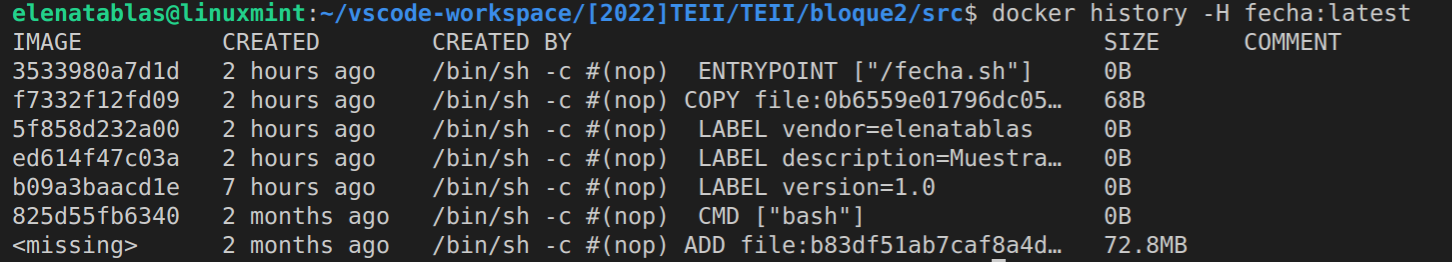
\includegraphics[width=\textwidth]{docker-history}
    \centering
    \caption{Capas de una imagen docker.}
    \label{fig:docker-histoy}
 \end{figure}
\par Las primeras dos capas son de la imagen oficial de \texttt{ubuntu}, las siguientes tres 
capas son varias etiquetas que he añadido que solo son informativas. Las dos últimas son 
para copiar un recurso y ejecutarlo sin tener que llamar al shell.
\par \textbf{Dockerfile1}
\begin{listing}
    # 2 capas de esta nueva imagen
    FROM ubuntu
    
    # Pueden ir en cualquier nivel de la imagen, normalmente al inicio
    LABEL version=1.0
    LABEL description="Muestra la fecha actual por pantalla cada segundo." 
    LABEL vendor=elenatablas
    
    COPY fecha.sh /fecha.sh
    ENTRYPOINT ["/fecha.sh"] 
\end{listing}

\par \textbf{fecha.sh}
\par Este script muestra la fecha cada segundo durante su ejecución.
\begin{listing}
    #!/bin/bash

    while true; do echo "$(date +%d/%m/%y)"; sleep 1; done 
\end{listing}
